\subsection{Analysis of the results}

\paragraph{}In this section, there are going to be presented several graphs with the different parameters that have been obtained in the simulation of the case. The following plots are the results of all the commands that have been mentioned in the previous sections and are divided into two sections


\subsubsection{Velocity}
\subsubsubsection{Overall look}

\begin{figure}[h!]
\centering
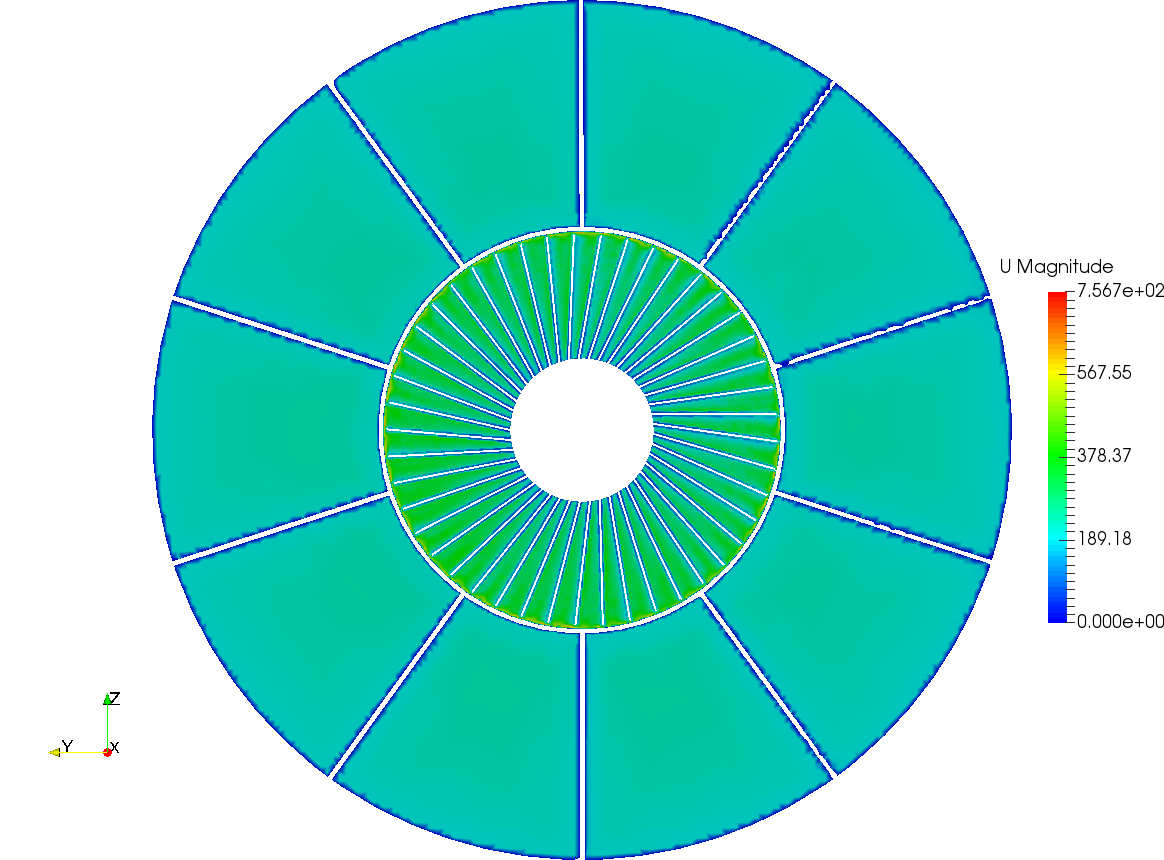
\includegraphics[scale=0.25]{./img/screenshoots/U1.png}
\caption{Total speed}
\label{u1}
\end{figure}

\begin{figure}[h!]
\centering
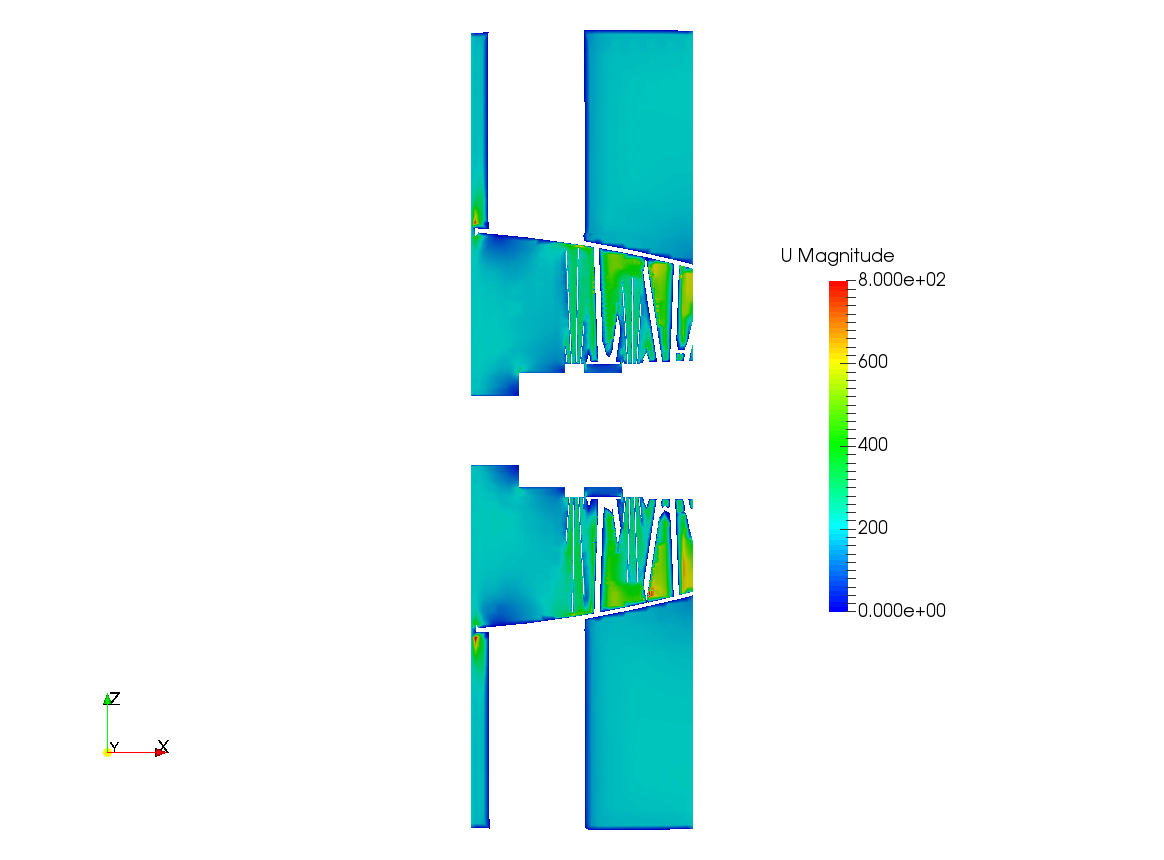
\includegraphics[scale=0.3]{./img/screenshoots/U2.png}
\caption{Total speed}
\label{u2}
\end{figure}


\begin{figure}[h!]
\centering
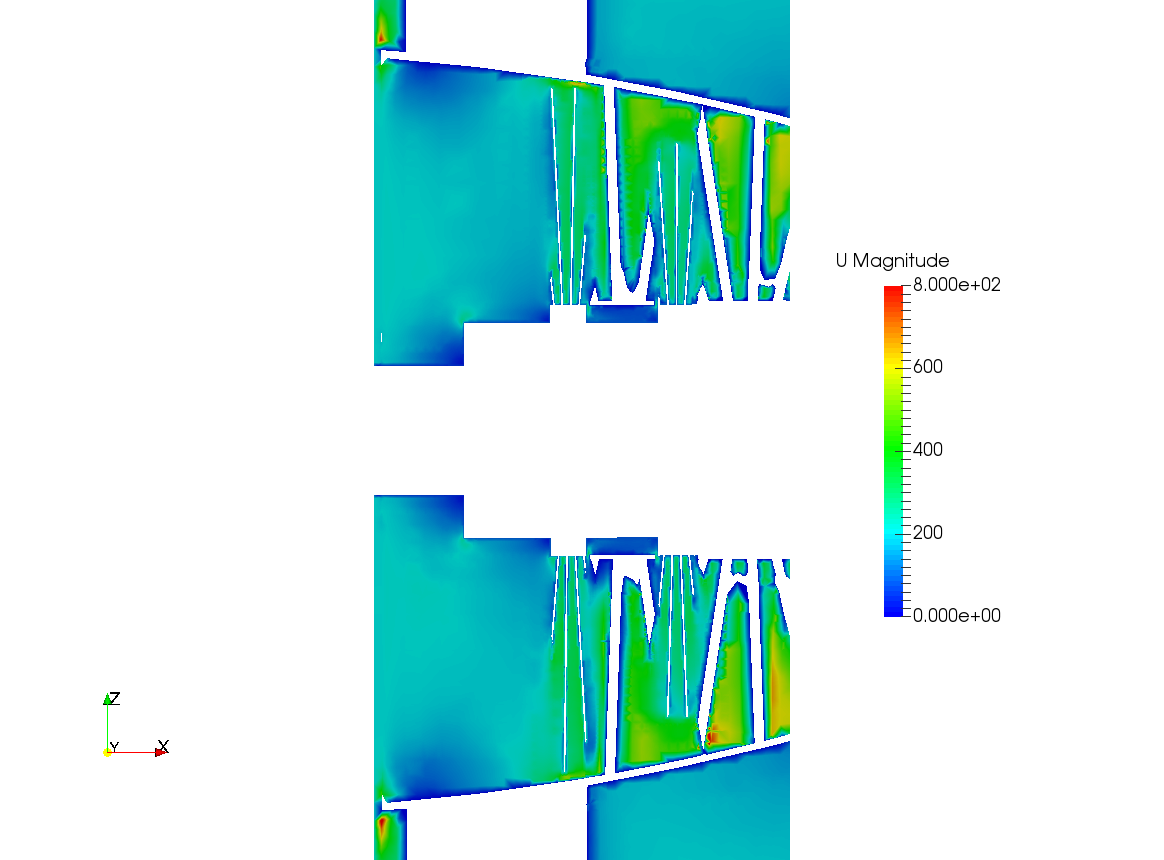
\includegraphics[scale=0.3]{./img/screenshoots/U2bis.png}
\caption{Detail of the total speed}
\label{u2bis}
\end{figure}


\newpage\subsubsubsection{Velocity in the x direction}

\begin{figure}[h!]
\centering
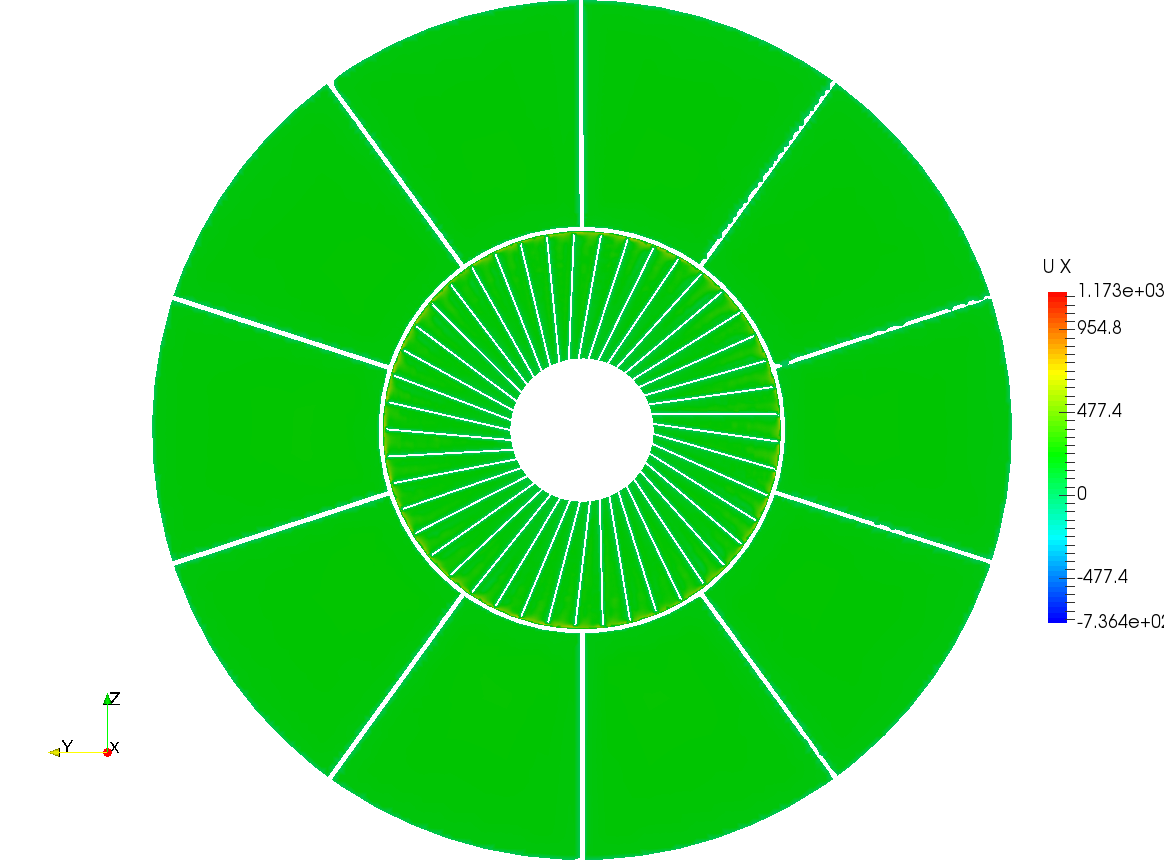
\includegraphics[scale=0.28]{./img/screenshoots/Ux1.png}
\caption{Speed in the x direction}
\label{ux1}
\end{figure}

\begin{figure}[h!]
\centering
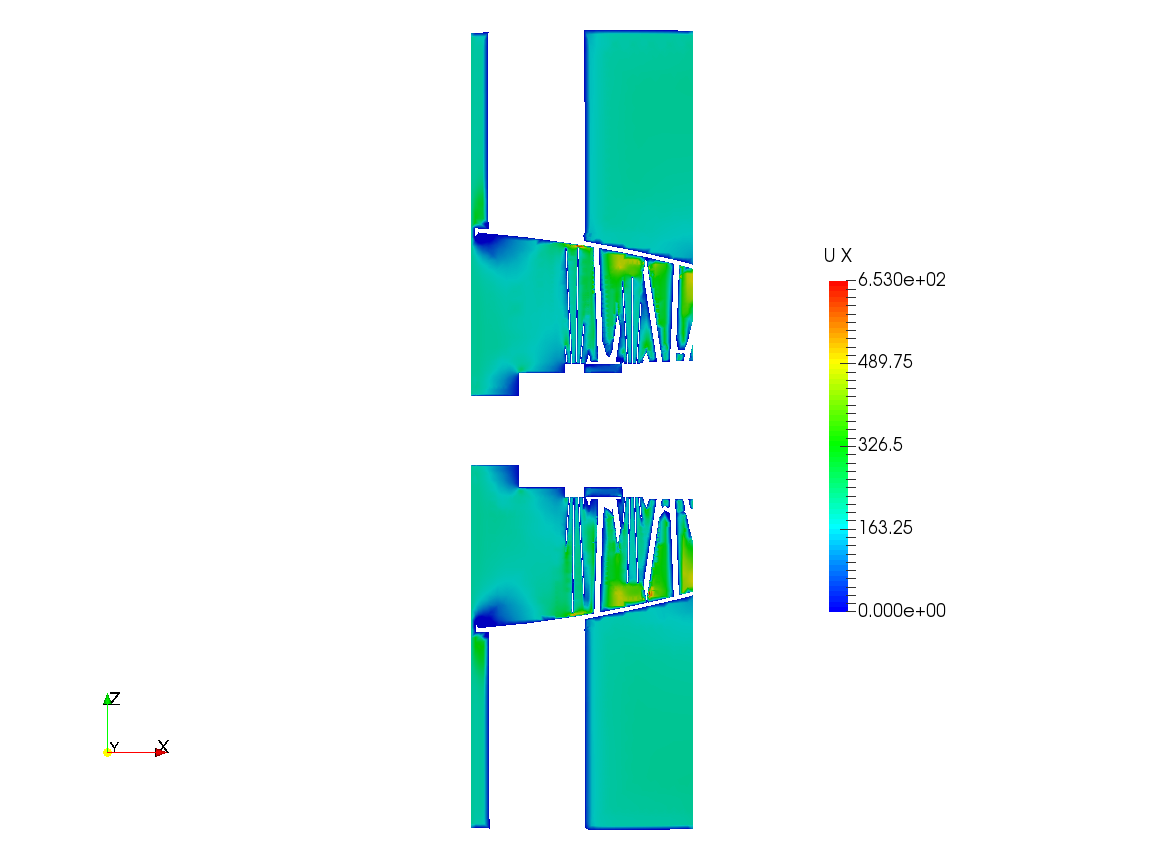
\includegraphics[scale=0.28]{./img/screenshoots/Ux2.png}
\caption{Speed in the x direction}
\label{ux2}
\end{figure}

\newpage\subsubsubsection{Velocity in the y direction}

\begin{figure}[h!]
\centering
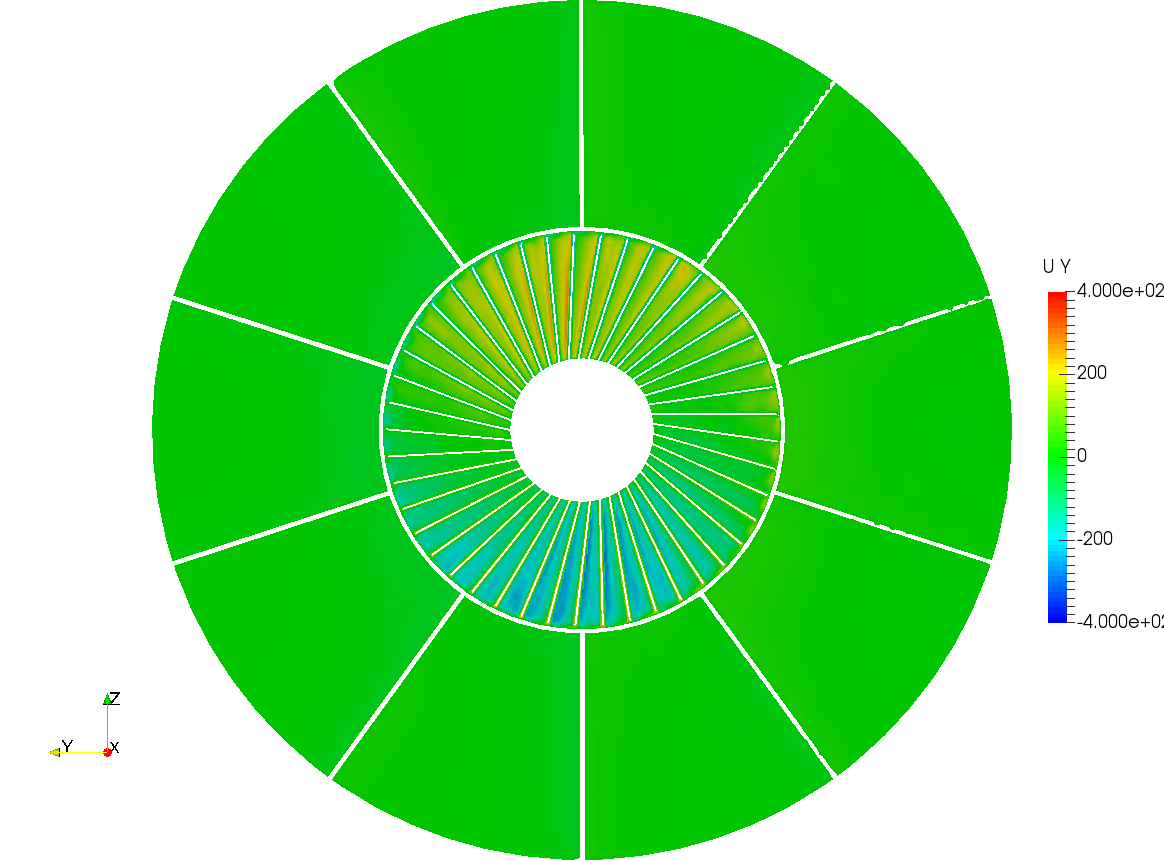
\includegraphics[scale=0.28]{./img/screenshoots/Uy1.png}
\caption{Speed in the y direction}
\label{uy1}
\end{figure}

\begin{figure}[h!]
\centering
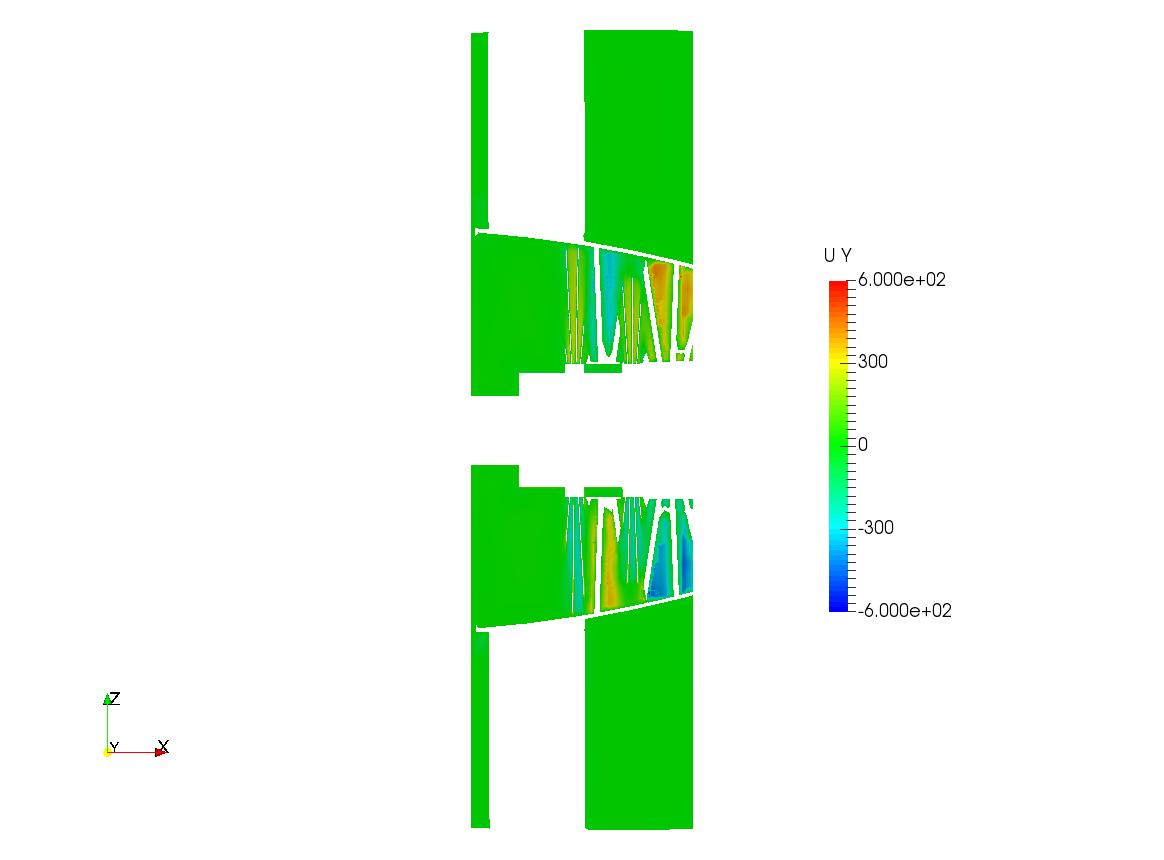
\includegraphics[scale=0.28]{./img/screenshoots/Uy2.png}
\caption{Speed in the y direction}
\label{uy2}
\end{figure}

\begin{figure}[h!]
\centering
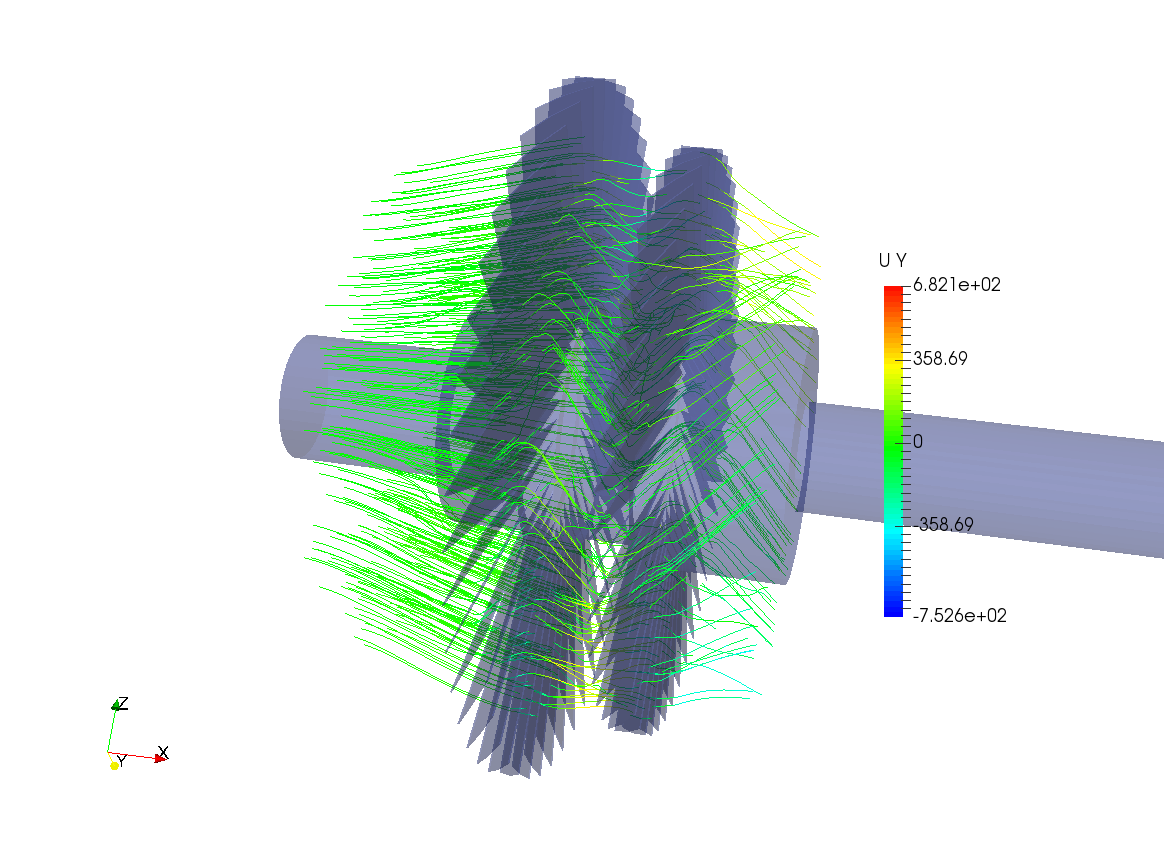
\includegraphics[scale=0.28]{./img/screenshoots/Uy3.png}
\caption{Stream lines in the y direction}
\label{uy3}
\end{figure}

\newpage\subsubsubsection{Velocity in the z direction}

\begin{figure}[h!]
\centering
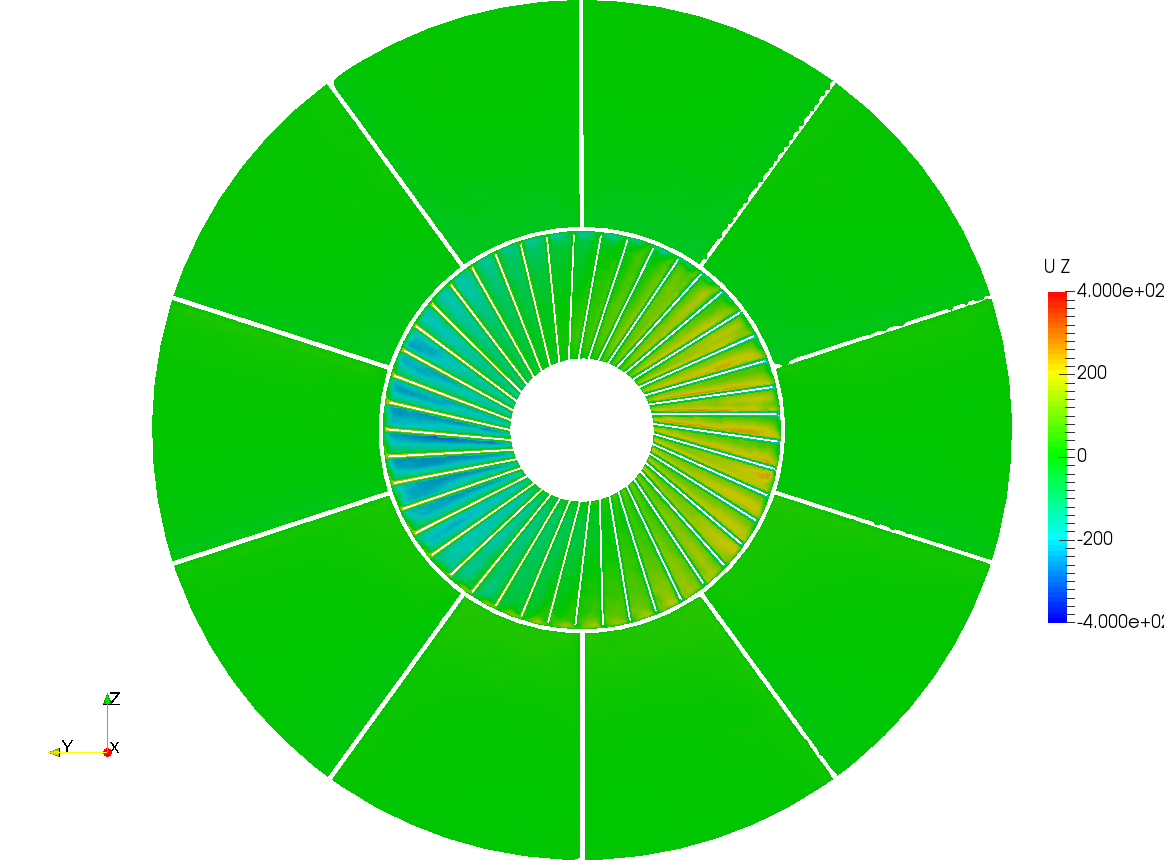
\includegraphics[scale=0.28]{./img/screenshoots/Uz1.png}
\caption{Speed in the z direction}
\label{uz1}
\end{figure}

\begin{figure}[h!]
\centering
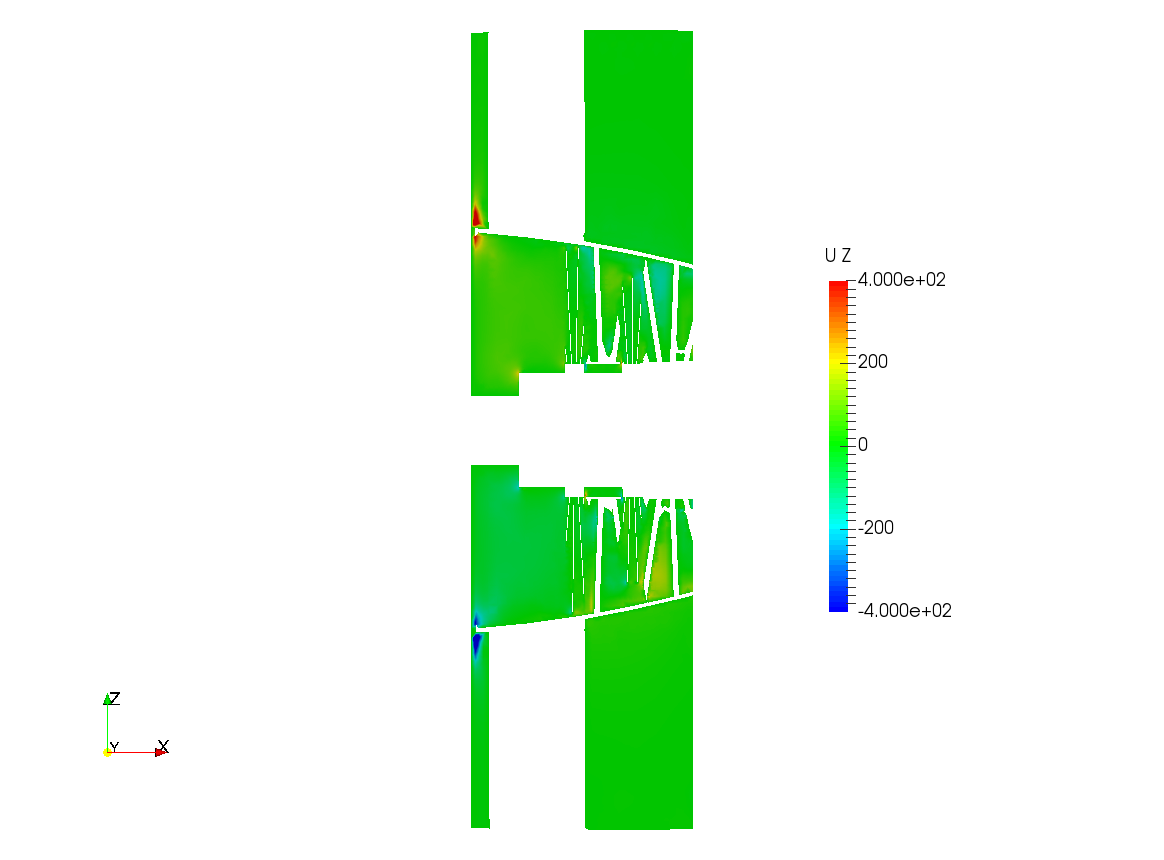
\includegraphics[scale=0.28]{./img/screenshoots/Uz2.png}
\caption{Speed in the z direction}
\label{uz2}
\end{figure}

\newpage\subsubsection{Pressure}

\begin{figure}[h!]
\centering
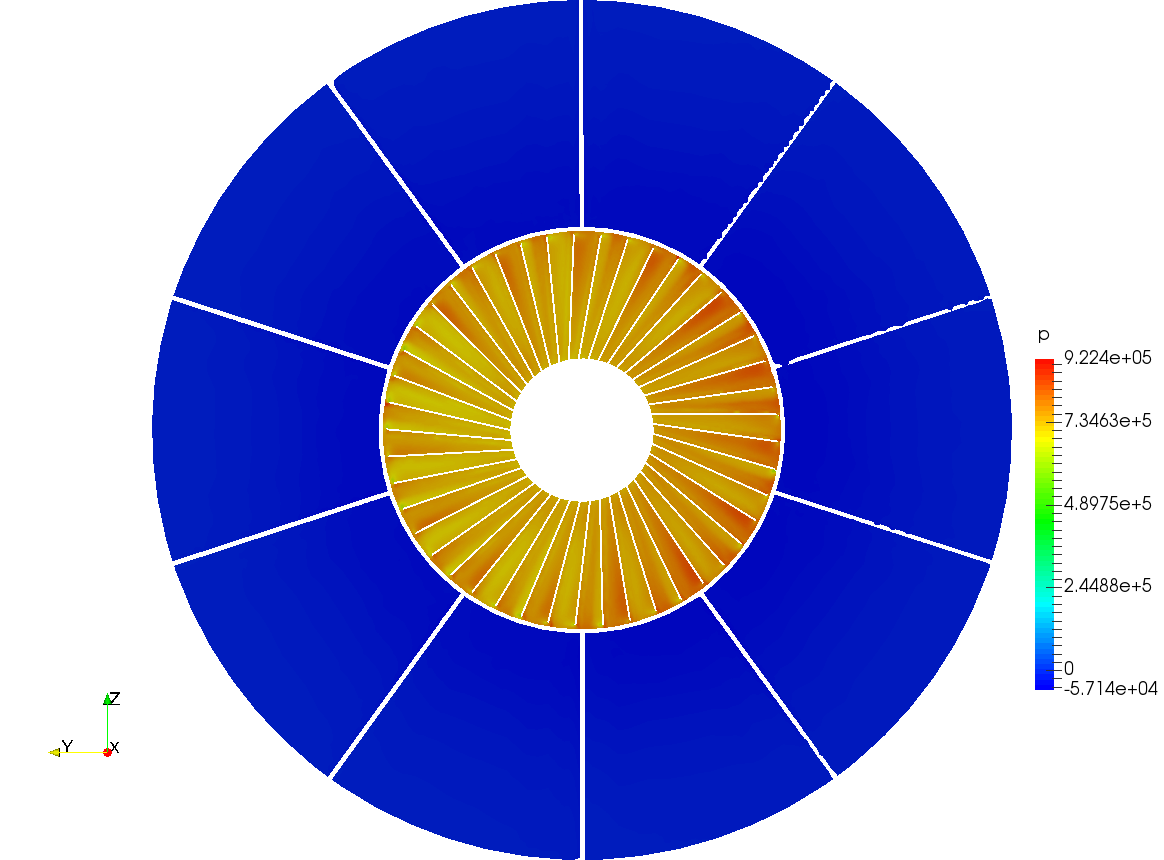
\includegraphics[scale=0.28]{./img/screenshoots/p1.png}
\caption{Pressure}
\label{p1}
\end{figure}

\begin{figure}[h!]
\centering
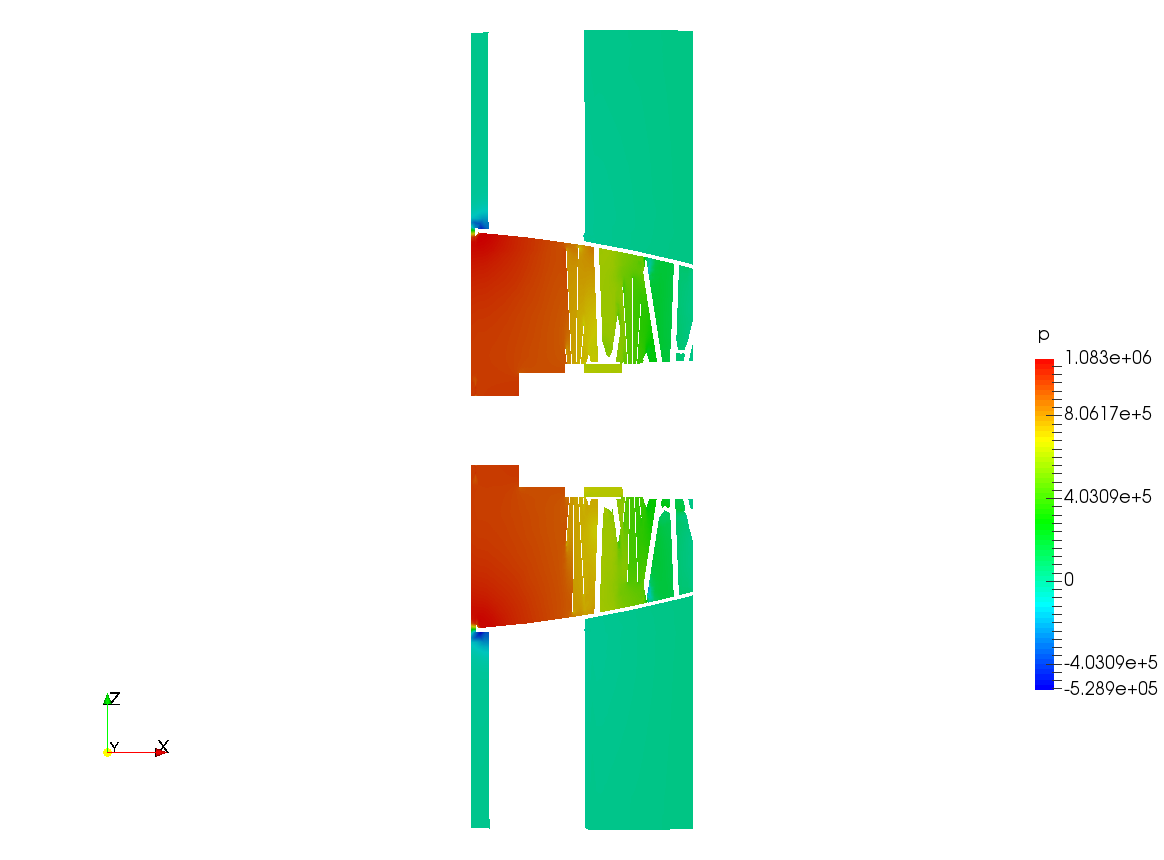
\includegraphics[scale=0.28]{./img/screenshoots/p2.png}
\caption{Pressure}
\label{p2}
\end{figure}

\newpage\subsubsection{Comments}
\paragraph{}In the first three images can be seen how th velocity increases as the flow travels through the compressor region. This is the expected behaviour since the velocity has to increae along with the pressure to achieve the maximum efficiency in the combustion chamber. It can be also seen that the velocity in the external ring remains unperturbed. This is because, this region is situated rear the fan and it only experiences the low-compression produced due to the fan blades.
\paragraph{}In the figures~\ref{ux1} and \ref{ux2} the distribution of the velocity in the X directon is shown. As one can simply see, the velcity does not change in its normal plane and the variation along the X direction is nearly the expected,achieving in the exit of this compression stage near $500 m/s$. 
\paragraph{}The next four figures show the evolution of the velocity in the Y and Z directions. It can be seen that the field rotates. The angular velocity can be also computed. Finally, the last two figures show the pressure field.